%chapter 16

\chapter{Clases y funciones}

Ahora que sabemos cómo crear nuevos tipos, el siguiente paso es escribir funciones que tomen objetos definidos por el programador como parámetros y los devuelvan como resultados. En este capítulo también presento el "estilo de programación funcional" y dos nuevos planes de desarrollo de programas.

Los ejemplos de código de este capítulo están disponibles en \url{https://thinkpython.com/code/Time1.py}. Las soluciones a los ejercicios se encuentran en \url{https://thinkpython.com/code/Time1_soln.py}.

\section{Tiempo}

Como otro ejemplo de un tipo definido por el programador, definiremos una clase llamada \texttt{Time} que registra la hora del día. La definición de la clase se ve así:

\begin{lstlisting}[language=Python]
class Time:
    """Representa la hora del día.
    atributos: hour, minute, second
    """
\end{lstlisting}

Podemos crear un nuevo objeto \texttt{Time} y asignar atributos para horas, minutos y segundos:

\begin{lstlisting}[language=Python]
time = Time()
time.hour = 11
time.minute = 59
time.second = 30
\end{lstlisting}

El diagrama de estado para el objeto \texttt{Time} se muestra en la Figura 16.1.

Como ejercicio, escribe una función llamada \texttt{print\_time} que tome un objeto \texttt{Time} y lo imprima en el formato \texttt{hour:minute:second}. Pista: la secuencia de formato \texttt{'\%02d'} imprime un entero usando al menos dos dígitos, incluyendo un cero inicial si es necesario.

Escribe una función booleana llamada \texttt{is\_after} que tome dos objetos \texttt{Time}, \texttt{t1} y \texttt{t2}, y devuelva \texttt{True} si \texttt{t1} sigue cronológicamente a \texttt{t2} y \texttt{False} en caso contrario. Desafío: no uses una sentencia \texttt{if}.

\begin{figure}[h]
\centering
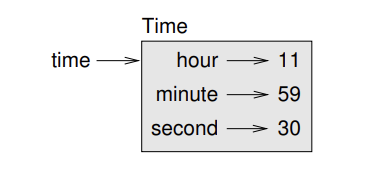
\includegraphics[width=0.5\textwidth]{./images/chapter_16_1.png}
\caption{Diagrama de objeto.}
\label{fig:time_diagram}
\end{figure}

\section{Funciones puras}

En las próximas secciones, escribiremos dos funciones que suman valores de tiempo. Estas demuestran dos tipos de funciones: funciones puras y modificadores. También demuestran un plan de desarrollo que llamaré "prototipo y parche", que es una forma de abordar un problema complejo comenzando con un prototipo simple y tratando las complicaciones de manera incremental.

Aquí hay un prototipo simple de \texttt{add\_time}:

\begin{lstlisting}[language=Python]
def add_time(t1, t2):
    sum = Time()
    sum.hour = t1.hour + t2.hour
    sum.minute = t1.minute + t2.minute
    sum.second = t1.second + t2.second
    return sum
\end{lstlisting}

La función crea un nuevo objeto \texttt{Time}, inicializa sus atributos y devuelve una referencia al nuevo objeto. Esto se llama una \textbf{función pura} porque no modifica ninguno de los objetos que se le pasan como argumentos y no tiene ningún efecto, como mostrar un valor u obtener entrada del usuario, aparte de devolver un valor.

Para probar esta función, crearé dos objetos \texttt{Time}: \texttt{start} contiene la hora de inicio de una película, como \textit{Monty Python and the Holy Grail}, y \texttt{duration} contiene la duración de la película, que es de una hora y 35 minutos.

\texttt{add\_time} calcula cuándo terminará la película.

\begin{lstlisting}[language=Python]
>>> start = Time()
>>> start.hour = 9
>>> start.minute = 45
>>> start.second = 0
>>> duration = Time()
>>> duration.hour = 1
>>> duration.minute = 35
>>> duration.second = 0
>>> done = add_time(start, duration)
>>> print_time(done)
10:80:00
\end{lstlisting}

El resultado, \texttt{10:80:00}, podría no ser lo que esperabas. El problema es que esta función no maneja los casos donde el número de segundos o minutos suma más de sesenta. Cuando eso sucede, tenemos que "llevar" los segundos extra a la columna de minutos o los minutos extra a la columna de horas.

Aquí hay una versión mejorada:

\begin{lstlisting}[language=Python]
def add_time(t1, t2):
    sum = Time()
    sum.hour = t1.hour + t2.hour
    sum.minute = t1.minute + t2.minute
    sum.second = t1.second + t2.second

    if sum.second >= 60:
        sum.second -= 60
        sum.minute += 1

    if sum.minute >= 60:
        sum.minute -= 60
        sum.hour += 1

    return sum
\end{lstlisting}

Aunque esta función es correcta, está empezando a crecer. Veremos una alternativa más corta más adelante.

\section{Modificadores}

A veces es útil que una función modifique los objetos que recibe como parámetros. En ese caso, los cambios son visibles para quien llama. Las funciones que funcionan así se llaman \textbf{modificadores}.

\texttt{increment}, que agrega una cantidad dada de segundos a un objeto \texttt{Time}, puede escribirse naturalmente como un modificador. Aquí hay un borrador:

\begin{lstlisting}[language=Python]
def increment(time, seconds):
    time.second += seconds

    if time.second >= 60:
        time.second -= 60
        time.minute += 1

    if time.minute >= 60:
        time.minute -= 60
        time.hour += 1
\end{lstlisting}

La primera línea realiza la operación básica; el resto maneja los casos especiales que vimos antes.

¿Es esta función correcta? ¿Qué pasa si \texttt{seconds} es mucho mayor que sesenta?

En ese caso, no es suficiente con llevar una vez; tenemos que seguir haciéndolo hasta que \texttt{time.second} sea menor que sesenta. Una solución es reemplazar las sentencias \texttt{if} con sentencias \texttt{while}. Eso haría que la función fuera correcta, pero no muy eficiente. Como ejercicio, escribe una versión correcta de \texttt{increment} que no contenga bucles.

Cualquier cosa que se pueda hacer con modificadores también se puede hacer con funciones puras. De hecho, algunos lenguajes de programación solo permiten funciones puras. Hay evidencia de que los programas que usan funciones puras se desarrollan más rápido y son menos propensos a errores que los programas que usan modificadores. Pero los modificadores son convenientes a veces, y los programas funcionales tienden a ser menos eficientes.

En general, recomiendo que escribas funciones puras siempre que sea razonable y recurras a modificadores solo si hay una ventaja convincente. Este enfoque podría llamarse \textbf{estilo de programación funcional}.

Como ejercicio, escribe una versión "pura" de \texttt{increment} que cree y devuelva un nuevo objeto \texttt{Time} en lugar de modificar el parámetro.

\section{Prototipado versus planificación}

El plan de desarrollo que estoy demostrando se llama "prototipo y parche". Para cada función, escribí un prototipo que realizaba el cálculo básico y luego lo probé, corrigiendo errores en el camino.

Este enfoque puede ser efectivo, especialmente si aún no tienes una comprensión profunda del problema. Pero las correcciones incrementales pueden generar código innecesariamente complicado (ya que maneja muchos casos especiales) y poco confiable (ya que es difícil saber si has encontrado todos los errores).

Una alternativa es el \textbf{desarrollo diseñado}, en el que una comprensión de alto nivel del problema puede hacer que la programación sea mucho más fácil. En este caso, la idea es que un objeto \texttt{Time} es en realidad un número de tres dígitos en base 60. El atributo \texttt{second} es la "columna de las unidades", el atributo \texttt{minute} es la "columna de los sesentas" y el atributo \texttt{hour} es la "columna de los tres mil seiscientos".

Cuando escribimos \texttt{add\_time} e \texttt{increment}, estábamos haciendo efectivamente una suma en base 60, razón por la cual teníamos que llevar de una columna a la siguiente.

Esta observación sugiere otro enfoque para todo el problema: podemos convertir objetos \texttt{Time} a enteros y aprovechar el hecho de que la computadora sabe cómo hacer aritmética con enteros.

Aquí hay una función que convierte \texttt{Time} a enteros:

\begin{lstlisting}[language=Python]
def time_to_int(time):
    minutes = time.hour * 60 + time.minute
    seconds = minutes * 60 + time.second
    return seconds
\end{lstlisting}

Y aquí hay una función que convierte un entero a \texttt{Time} (recuerda que \texttt{divmod} divide el primer argumento por el segundo y devuelve el cociente y el resto como una tupla):

\begin{lstlisting}[language=Python]
def int_to_time(seconds):
    time = Time()
    minutes, time.second = divmod(seconds, 60)
    time.hour, time.minute = divmod(minutes, 60)
    return time
\end{lstlisting}

Podrías tener que pensar un poco y ejecutar algunas pruebas para convencerte de que estas funciones son correctas. Una forma de probarlas es verificar que \texttt{time\_to\_int(int\_to\_time(x)) == x} para muchos valores de \texttt{x}. Este es un ejemplo de una verificación de consistencia.

Una vez que estés convencido de que son correctas, puedes usarlas para reescribir \texttt{add\_time}:

\begin{lstlisting}[language=Python]
def add_time(t1, t2):
    seconds = time_to_int(t1) + time_to_int(t2)
    return int_to_time(seconds)
\end{lstlisting}

Esta versión es más corta que la original y más fácil de verificar. Como ejercicio, reescribe \texttt{increment} usando \texttt{time\_to\_int} e \texttt{int\_to\_time}.

En algunos aspectos, convertir de base 60 a base 10 y viceversa es más difícil que simplemente lidiar con valores de tiempo. La conversión de base es más abstracta; nuestra intuición para manejar valores de tiempo es mejor.

Pero si tenemos la idea de tratar los tiempos como números en base 60 y hacemos el esfuerzo de escribir las funciones de conversión (\texttt{time\_to\_int} e \texttt{int\_to\_time}), obtenemos un programa que es más corto, más fácil de leer y depurar, y más confiable.

También es más fácil agregar características más adelante. Por ejemplo, imagina restar dos \texttt{Time} para encontrar la duración entre ellos. El enfoque ingenuo sería implementar la resta con préstamo. Usar las funciones de conversión sería más fácil y más probable que sea correcto.

Irónicamente, a veces hacer un problema más difícil (o más general) lo hace más fácil (porque hay menos casos especiales y menos oportunidades de error).

\section{Depuración}

Un objeto \texttt{Time} está bien formado si los valores de \texttt{minute} y \texttt{second} están entre 0 y 60 (incluyendo 0 pero no 60) y si \texttt{hour} es positivo. \texttt{hour} y \texttt{minute} deben ser valores enteros, pero podríamos permitir que \texttt{second} tenga una parte fraccionaria.

Requisitos como estos se llaman \textbf{invariantes} porque siempre deben ser verdaderos. Dicho de otra manera, si no son verdaderos, algo ha salido mal.

Escribir código para verificar invariantes puede ayudar a detectar errores y encontrar sus causas. Por ejemplo, podrías tener una función como \texttt{valid\_time} que toma un objeto \texttt{Time} y devuelve \texttt{False} si viola un invariante:

\begin{lstlisting}[language=Python]
def valid_time(time):
    if time.hour < 0 or time.minute < 0 or time.second < 0:
        return False
    if time.minute >= 60 or time.second >= 60:
        return False
    return True
\end{lstlisting}

Al comienzo de cada función, podrías verificar los argumentos para asegurarte de que son válidos:

\begin{lstlisting}[language=Python]
def add_time(t1, t2):
    if not valid_time(t1) or not valid_time(t2):
        raise ValueError('invalid Time object in add_time')
    seconds = time_to_int(t1) + time_to_int(t2)
    return int_to_time(seconds)
\end{lstlisting}

O podrías usar una \textbf{sentencia assert}, que verifica un invariante dado y genera una excepción si falla:

\begin{lstlisting}[language=Python]
def add_time(t1, t2):
    assert valid_time(t1) and valid_time(t2)
    seconds = time_to_int(t1) + time_to_int(t2)
    return int_to_time(seconds)
\end{lstlisting}

Las sentencias \texttt{assert} son útiles porque distinguen el código que maneja condiciones normales del código que verifica errores.

\section{Glosario}

\begin{description}
\item[prototipo y parche:] Un plan de desarrollo que implica escribir un borrador de un programa, probarlo y corregir errores a medida que se encuentran.
\item[desarrollo diseñado:] Un plan de desarrollo que implica una comprensión de alto nivel del problema y más planificación que el desarrollo incremental o el desarrollo de prototipos.
\item[función pura:] Una función que no modifica ninguno de los objetos que recibe como argumentos. La mayoría de las funciones puras son fructíferas.
\item[modificador:] Una función que cambia uno o más de los objetos que recibe como argumentos. La mayoría de los modificadores son nulos; es decir, devuelven \texttt{None}.
\item[estilo de programación funcional:] Un estilo de diseño de programas en el que la mayoría de las funciones son puras.
\item[invariante:] Una condición que siempre debe ser verdadera durante la ejecución de un programa.
\item[sentencia assert:] Una sentencia que verifica una condición y genera una excepción si falla.
\end{description}

\section{Ejercicios}

Los ejemplos de código de este capítulo están disponibles en \url{https://thinkpython.com/code/Time1.py}; las soluciones a los ejercicios están disponibles en \url{https://thinkpython.com/code/Time1_soln.py}.

\begin{enumerate}
\item \textbf{Ejercicio 16.1.} Escribe una función llamada \texttt{mul\_time} que tome un objeto \texttt{Time} y un número y devuelva un nuevo objeto \texttt{Time} que contenga el producto del \texttt{Time} original y el número.

Luego usa \texttt{mul\_time} para escribir una función que tome un objeto \texttt{Time} que represente el tiempo de finalización en una carrera y un número que represente la distancia, y devuelva un objeto \texttt{Time} que represente el ritmo promedio (tiempo por milla).

\item \textbf{Ejercicio 16.2.} El módulo \texttt{datetime} proporciona objetos de tiempo similares a los objetos \texttt{Time} de este capítulo, pero ofrecen un conjunto rico de métodos y operadores. Lee la documentación en \url{http://docs.python.org/3/library/datetime.html}.

\begin{enumerate}
\item Usa el módulo \texttt{datetime} para escribir un programa que obtenga la fecha actual e imprima el día de la semana.
\item Escribe un programa que tome un cumpleaños como entrada e imprima la edad del usuario y el número de días, horas, minutos y segundos hasta su próximo cumpleaños.
\item Para dos personas nacidas en días diferentes, hay un día en el que uno es el doble de viejo que el otro. Ese es su "Día Doble". Escribe un programa que tome dos fechas de nacimiento y calcule su Día Doble.
\item Para un poco más de desafío, escribe la versión más general que calcule el día en el que una persona es $n$ veces mayor que la otra.
\end{enumerate}

Solución: \url{https://thinkpython.com/code/double.py}
\end{enumerate}